\section{Signaldecoder}\label{text:Entwicklung-des-Stellwerks:Signaldecoder}

Wie zuvor bereits erwähnt, wurde der Signaldecoder aufgrund von Problemen mit der Kommunikation zwischen den Komponenten nicht implementiert. Er soll daher hier konzeptuell beschrieben werden.

Der Signaldecoder ist ein vergleichsweise simple Software, die auf einem Raspberry Pi Pico läuft. An diesem sind die LEDs aller Signale direkt angeschlossen (freilich mit einem passenden Widerstand). Initial wird dem Decoder von der zentralen Steuerung die Zuordnung von Signalen und I/O-Pins übermittelt. Danach kann er Befehle zum Stellen der Signale empfangen.

\begin{figure}[H]
    \centering
    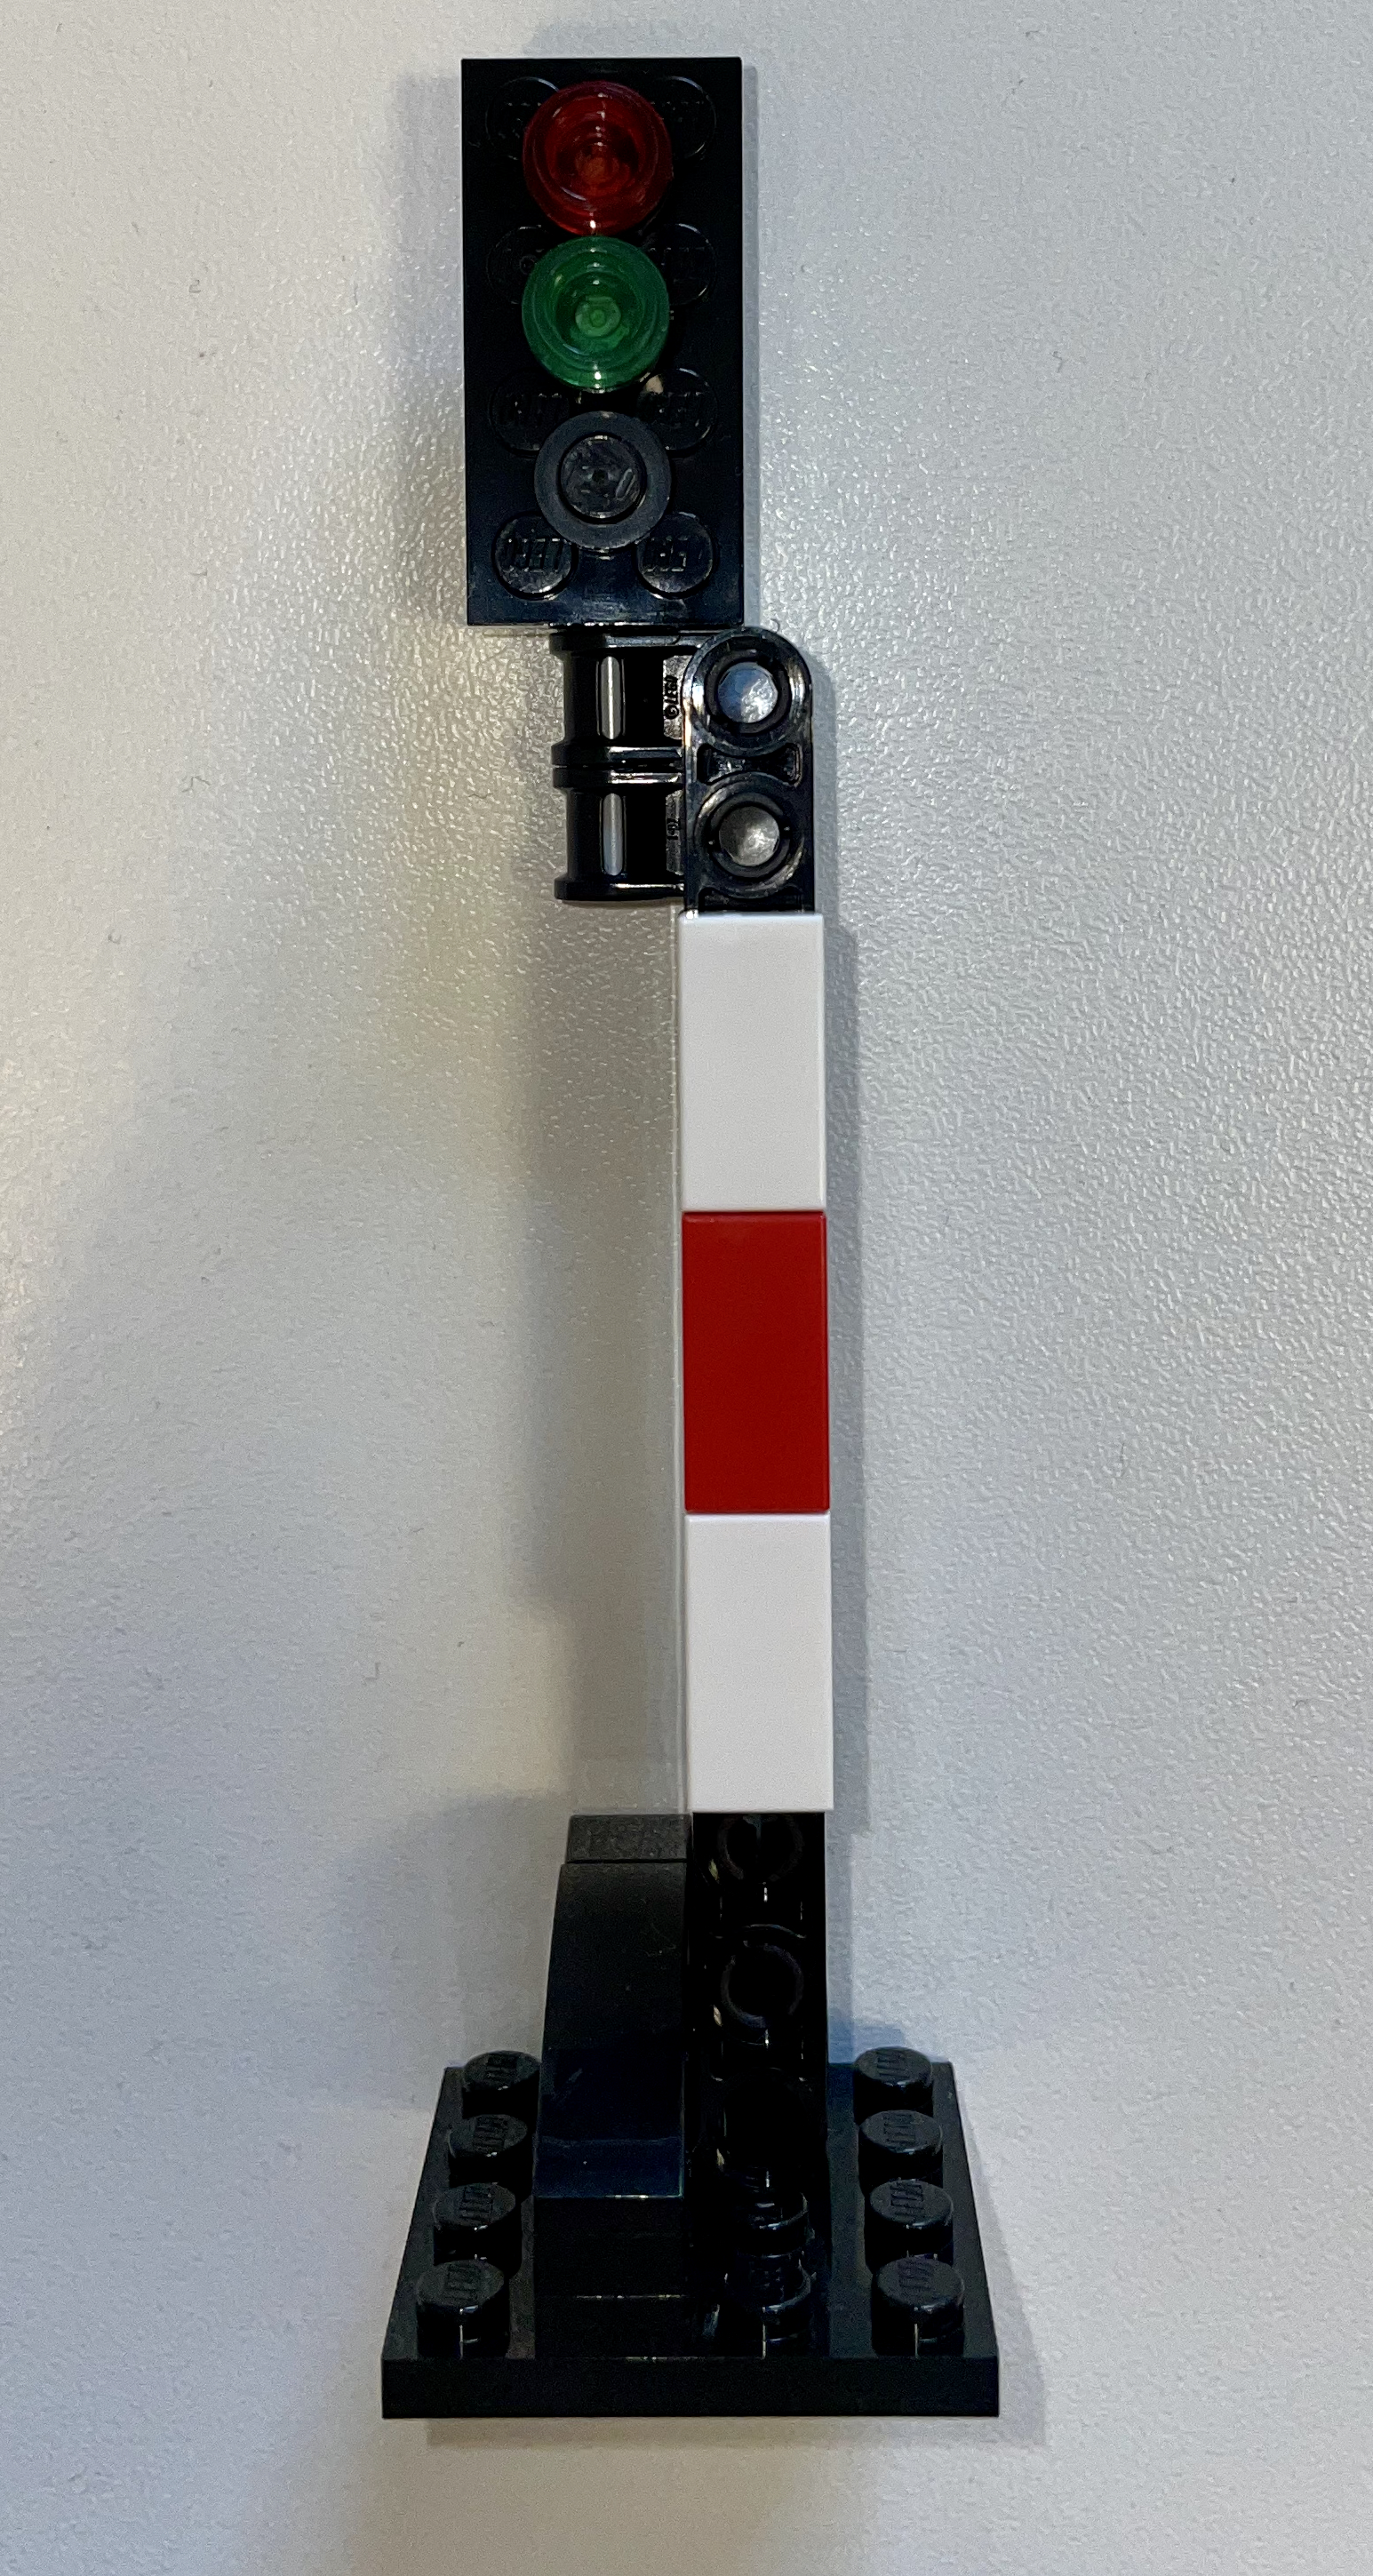
\includegraphics[width=.4\textwidth]{Assets/Images/5-Entwicklung-des-Stellwerks/Signal.jpg}
    \caption{Klemmbaustein-Signal}\label{abb:Entwicklung-des-Stellwerks:Signal}
\end{figure}

Sofern die Signale des Stellwerks nur zwei Signalbilder darstellen sollen, also \textit{Halt!} und \textit{Fahrt!}, werden nur zwei LEDs pro Signal benötigt, wobei nur eins von beiden gleichzeitig leuchten kann. In diesem Fall kann durch die Verwendung eines Wechsler-Relais die Anzahl von Signalen, die ein Decoder steuern kann, verdoppelt werden, da nur noch ein I/O-Pin zur Steuerung benötigt wird.
